\chapter{Joint and Conditional Entropy}
\label{ch:joint_conditional}

\section{The Geometry of Intersecting Uncertainties}

If the previous chapter dealt with the uncertainty of a single isolated event, this chapter deals with the reality of the physical world: events are almost never isolated. The sky being cloudy is not independent of whether it will rain. The pixel in the upper-left corner of an image is not independent of the pixel next to it. The entire premise of machine learning is built upon exploiting these dependencies. If variables were truly independent, prediction would be impossible.

To build neural networks that can predict $\mathcal{Y}$ from $\mathcal{X}$, we must first understand how to measure the joint uncertainty of multiple variables, and crucially, how the knowledge of one variable reduces the uncertainty of another. This brings us to the concepts of joint entropy and conditional entropy. 

Imagine two random variables as two overlapping shadows cast on a wall. The total area covered by both shadows represents their joint entropy---the total uncertainty when considering both variables together. The area where they overlap represents the information they share. The area of one shadow that is not covered by the other represents the conditional entropy---the remaining uncertainty in one variable after the other is fully known. 

In deep learning, this geometry of intersecting uncertainties is what we navigate during training. When an encoder network $q_\phi(z|x)$ maps an input $x$ to a latent representation $z$, we are acutely interested in the conditional entropy $H(Z|X)$. If the encoder is deterministic, this conditional entropy is zero. If it is stochastic, as in Variational Autoencoders, this conditional entropy represents the noise injected into the representation. Understanding how uncertainties combine and condition one another is the prerequisite for understanding mutual information, which we will tackle in the next chapter.

\section{Mathematical Definitions}

We begin by extending our definition of entropy to multiple variables. Let $X$ and $Y$ be discrete random variables drawn from alphabets $\mathcal{X}$ and $\mathcal{Y}$, respectively, with a joint probability mass function $p(x, y) = \text{Pr}(X=x, Y=y)$.

\begin{definition}[Joint Entropy]
The joint entropy $H(X, Y)$ of a pair of discrete random variables $(X, Y)$ is defined as the expected surprisal of their joint outcomes:
\begin{equation}
    H(X, Y) = -\sum_{x \in \mathcal{X}} \sum_{y \in \mathcal{Y}} p(x, y) \log p(x, y)
\end{equation}
\end{definition}

Joint entropy measures the total uncertainty needed to describe both $X$ and $Y$ simultaneously. It is straightforward to see that if $X$ and $Y$ are completely independent, meaning $p(x, y) = p(x)p(y)$ for all $x$ and $y$, then the logarithm splits, and $H(X, Y) = H(X) + H(Y)$. The uncertainties simply add up.

However, when variables are dependent, knowing one tells us something about the other. This remaining uncertainty is formalized as conditional entropy.

\begin{definition}[Conditional Entropy]
The conditional entropy $H(Y|X)$ of a random variable $Y$ given another random variable $X$ is the expected value of the entropies of the conditional distributions $p(y|x)$, averaged over the distribution of $x$:
\begin{equation}
    H(Y|X) = \sum_{x \in \mathcal{X}} p(x) H(Y | X=x) = -\sum_{x \in \mathcal{X}} \sum_{y \in \mathcal{Y}} p(x, y) \log p(y|x)
\end{equation}
\end{definition}

This definition is crucial. It answers the question: ``If I already know $X$, how much uncertainty still remains about $Y$ on average?'' 

\begin{theorem}[Chain Rule of Entropy]
\label{thm:chain_rule}
The joint entropy of $X$ and $Y$ is the entropy of $X$ plus the conditional entropy of $Y$ given $X$:
\begin{equation}
    H(X, Y) = H(X) + H(Y|X)
\end{equation}
\end{theorem}

\begin{proof}
By the definition of conditional probability, $p(x, y) = p(x)p(y|x)$. Substituting this into the definition of joint entropy:
\begin{align*}
    H(X, Y) &= -\sum_{x \in \mathcal{X}} \sum_{y \in \mathcal{Y}} p(x, y) \log p(x, y) \\
    &= -\sum_{x \in \mathcal{X}} \sum_{y \in \mathcal{Y}} p(x, y) \log \left( p(x) p(y|x) \right) \\
    &= -\sum_{x \in \mathcal{X}} \sum_{y \in \mathcal{Y}} p(x, y) \log p(x) - \sum_{x \in \mathcal{X}} \sum_{y \in \mathcal{Y}} p(x, y) \log p(y|x) \\
    &= -\sum_{x \in \mathcal{X}} p(x) \log p(x) \underbrace{\sum_{y \in \mathcal{Y}} p(y|x)}_{1} + H(Y|X) \\
    &= H(X) + H(Y|X)
\end{align*}
The proof demonstrates how total uncertainty is built sequentially.
\end{proof}

\begin{corollary}[Conditioning Reduces Entropy]
For any two random variables $X$ and $Y$:
\begin{equation}
    H(Y|X) \leq H(Y)
\end{equation}
with equality if and only if $X$ and $Y$ are independent.
\end{corollary}
This confirms our intuition: knowing $X$ can only ever decrease (or leave unchanged) our uncertainty about $Y$. It can never increase it. Information is always non-negative.

\subsection{Worked Numerical Example}

Consider a dataset $\mathcal{D}$ where instances are either cats or dogs (variable $Y$), and they wear collars or do not (variable $X$). The joint distribution $p(x, y)$ is given by the following table:

\begin{center}
\begin{tabular}{c|cc|c}
 & $Y = \text{Dog}$ & $Y = \text{Cat}$ & Marginal $p(x)$ \\
\hline
$X = \text{Collar}$ & 0.4 & 0.1 & 0.5 \\
$X = \text{No Collar}$ & 0.2 & 0.3 & 0.5 \\
\hline
Marginal $p(y)$ & 0.6 & 0.4 & 1.0
\end{tabular}
\end{center}

First, let's calculate the marginal entropies $H(X)$ and $H(Y)$:
\begin{align*}
    H(X) &= - (0.5 \log_2 0.5 + 0.5 \log_2 0.5) = 1 \text{ bit} \\
    H(Y) &= - (0.6 \log_2 0.6 + 0.4 \log_2 0.4) \approx 0.971 \text{ bits}
\end{align*}

Next, the joint entropy $H(X, Y)$:
\begin{align*}
    H(X, Y) &= - (0.4 \log_2 0.4 + 0.1 \log_2 0.1 + 0.2 \log_2 0.2 + 0.3 \log_2 0.3) \\
    &\approx 0.529 + 0.332 + 0.464 + 0.521 = 1.846 \text{ bits}
\end{align*}

Now, let's calculate the conditional entropy $H(Y|X)$. We need the conditional distributions $p(y|x) = p(x, y)/p(x)$:
For $X = \text{Collar}$: $p(\text{Dog}|\text{Collar}) = 0.4/0.5 = 0.8$, $p(\text{Cat}|\text{Collar}) = 0.2$.
For $X = \text{No Collar}$: $p(\text{Dog}|\text{No Collar}) = 0.2/0.5 = 0.4$, $p(\text{Cat}|\text{No Collar}) = 0.6$.

\begin{align*}
    H(Y|X=\text{Collar}) &= - (0.8 \log_2 0.8 + 0.2 \log_2 0.2) \approx 0.722 \text{ bits} \\
    H(Y|X=\text{No Collar}) &= - (0.4 \log_2 0.4 + 0.6 \log_2 0.6) \approx 0.971 \text{ bits}
\end{align*}

Averaging these over $p(x)$:
\begin{align*}
    H(Y|X) &= 0.5 \times 0.722 + 0.5 \times 0.971 \\
    &= 0.361 + 0.4855 = 0.8465 \text{ bits}
\end{align*}

We can verify the chain rule: $H(X) + H(Y|X) = 1 + 0.8465 = 1.8465 \approx H(X, Y)$.
Notice that $H(Y|X) = 0.8465 < H(Y) = 0.971$. Knowing whether the animal has a collar reduces our uncertainty about whether it is a dog or a cat.

\begin{figure}[ht]
    \centering
    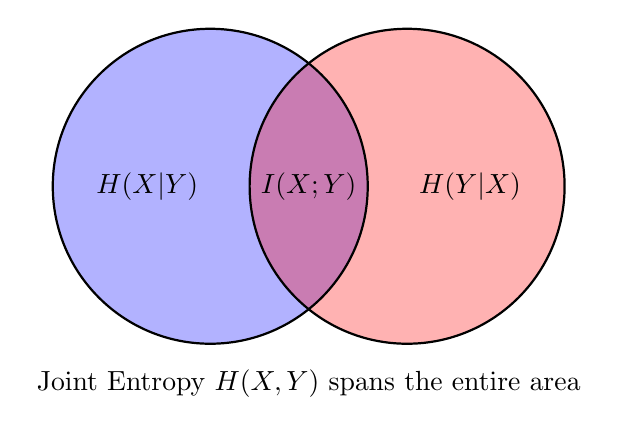
\begin{tikzpicture}
      % Left circle (X)
      \fill[blue, opacity=0.3] (0,0) circle (2cm);
      % Right circle (Y)
      \fill[red, opacity=0.3] (2.5,0) circle (2cm);
      
      % Outlines
      \draw[thick] (0,0) circle (2cm);
      \draw[thick] (2.5,0) circle (2cm);
      
      % Labels
      \node at (-0.8, 0) {$H(X|Y)$};
      \node at (3.3, 0) {$H(Y|X)$};
      \node at (1.25, 0) {$I(X;Y)$};
      
      % Overall label
      \node at (1.25, -2.5) {Joint Entropy $H(X,Y)$ spans the entire area};
    \end{tikzpicture}
    \caption{Information Venn Diagram. The total area represents the joint entropy $H(X,Y)$. The non-overlapping regions are the conditional entropies, while the intersection is the mutual information.}
    \label{fig:venn}
\end{figure}

\begin{figure}[ht]
    \centering
    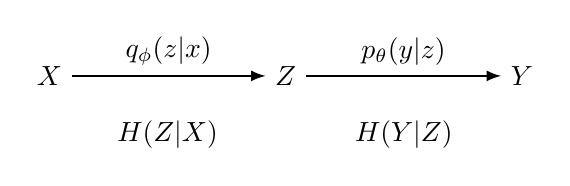
\begin{tikzpicture}[>=latex, scale=1.5]
        % Nodes
        \node (x) at (0, 0) {$X$};
        \node (z) at (2, 0) {$Z$};
        \node (y) at (4, 0) {$Y$};
        
        % Arrows
        \draw[->, thick] (x) -- (z) node[midway, above] {$q_\phi(z|x)$};
        \draw[->, thick] (z) -- (y) node[midway, above] {$p_\theta(y|z)$};
        
        % Annotations
        \node at (1, -0.5) {$H(Z|X)$};
        \node at (3, -0.5) {$H(Y|Z)$};
    \end{tikzpicture}
    \caption{A Markov chain in a typical representation learning setup. The conditional entropy $H(Z|X)$ dictates the stochasticity of the encoder.}
    \label{fig:markov_encoder}
\end{figure}

In the context of deep learning (Figure~\ref{fig:markov_encoder}), when we feed data $x$ into a neural network to produce a representation $z$, we are defining a conditional distribution $q_\phi(z|x)$. If this mapping is a standard deterministic feedforward network, then $p(z|x) = 1$ for the specific output and $0$ otherwise. Consequently, the conditional entropy $H(Z|X) = 0$. However, in models like Variational Autoencoders \cite{kingma2013auto}, the encoder maps to a Gaussian distribution, making $H(Z|X) > 0$. This non-zero conditional entropy acts as a regularizer, forcing the network to smooth its representations and preventing it from memorizing the exact input $x$.

\begin{horizon}
The mathematical bedrock of conditional entropy is universally accepted for discrete and well-behaved continuous distributions. However, deep neural networks routinely process highly dimensional data where the true joint distribution $P_{\text{data}}(X,Y)$ is unknown and arguably uncomputable. 

It is conjectured that the implicit bias of optimization algorithms like SGD biases networks toward representations $Z$ that minimize the conditional entropy $H(Y|Z)$ (maximizing predictive accuracy) while simultaneously, and perhaps inadvertently, increasing $H(Z|X)$ by flattening local minima in the parameter space. This suggests a thermodynamic tradeoff between the precision of the output and the ``heat'' or noise tolerated in the internal representation.

An open question is how to rigorously quantify $H(Z|X)$ when $f_\theta$ is formally deterministic (hence $H(Z|X)=0$ in Shannon's sense), but highly sensitive to imperceptible input noise, as seen in adversarial examples. Can conditional entropy be redefined topologically or geometrically on the data manifold to reflect this practical fragility? Future research into information geometry might bridge this gap by treating adversarial robustness as a constraint on the empirical conditional entropy.
\end{horizon}

\section*{Summary}
In this chapter, we expanded our view from single variables to interacting systems. Joint entropy $H(X,Y)$ quantifies the total uncertainty of a system, while conditional entropy $H(Y|X)$ measures the remaining uncertainty in $Y$ when $X$ is known. We proved the Chain Rule of Entropy, demonstrating how uncertainties aggregate. Finally, we saw how conditional entropy acts as a measure of stochasticity in neural network encoders, serving as a critical control knob in generative modeling.

\section*{Exercises}
\begin{enumerate}
    \item \textbf{Symmetry:} Prove that $H(X,Y) = H(Y,X)$ and interpret this result. Does $H(X|Y) = H(Y|X)$? Give a counterexample if false.
    \item \textbf{Deterministic Functions:} If $Y = f(X)$ where $f$ is a deterministic function, prove that $H(Y|X) = 0$. Then prove that $H(X,Y) = H(X)$.
    \item \textbf{Chain Rule for N Variables:} Extend Theorem~\ref{thm:chain_rule} to three variables, expressing $H(X,Y,Z)$ in terms of individual conditional entropies.
    \item \textbf{Network Encoders:} Let $x$ be an image and $z = q_\phi(x)$ be a latent vector. If $q_\phi$ adds isotropic Gaussian noise $\mathcal{N}(0, \sigma^2 I)$ to the output, write an expression for $H(Z|X)$. How does $\sigma$ affect the model's capacity to memorize $x$?
    \item \textbf{Data Processing:} If $X \to Y \to Z$ form a Markov chain, prove that $H(Z|X) \leq H(Z|Y)$ is generally false. Construct a counterexample.
\end{enumerate}
